%% Pre�mbulo -------------------------------------------


\documentclass[english,spanish,aspectratio=169,11 pt,utf8]{beamer}	% Establecer la clase de documento (Beamer), el tama�o de letra (9 puntos) y ancho de p�gina
\usepackage[spanish]{babel}
\selectlanguage{spanish}
\usepackage[utf8]{inputenc}
\usepackage[T1]{fontenc}										% Establecer el codificador de fuente (T1 [fuente EC] permite un �pima separaci�n sil�bica)
\usepackage{ae,aecompl}											% Usar la versi�n Tipo 1 de la fuente EC (Fuente: http://dsanta.users.ch/resources/type1.html)
\setcounter{secnumdepth}{3}										% Establecer el nivel profundidad que aparecen en los t�tulos de las secciones numeradas (secnum)
\setcounter{tocdepth}{3}										% Establecer el nivel profundidad que aparecen en la tabla de contenidos (toc)
\setlength{\parskip}{\smallskipamount}							% Establecer una separaci�n de p�rrafos peque�a
\setlength{\parindent}{0pt}										% Establecer un tama�o de sangr�a en todo el documento (en esta caso no hay sangr�a)
\usepackage{amsmath}											% Mejoras en las salidas matem�ticas del documento (American Mathematical Society)
\usepackage{mathtools}											% Mejoras de apariencia del documento con mucho contenido matem�tico (arregla problemas de amsmath)
\usepackage{amsthm}												% Es una extensi�n para el \newtheorem command de LaTeX (American Mathematical Society)
\usepackage{cancel}												% Permite trazar un l�nea diagonal (slash) sobre un t�rmino matem�tico (cancelarlo)
\usepackage{lastpage}											% Permite tener enumeraci�n de p�ginas
\usepackage{wrapfig}											% Permite envolver texto en las im�genes
\usepackage{multirow}											% Permite juntar dos a m�s filas en un sola
\usepackage{caption}											% Permite poner t�tulo a las tablas
%%\usepackage{subcaption}										% Permite poner t�tulo a las sub-im�genes
\usepackage{graphicx}											% Contiene opciones respecto al manejo de im�genes
\usepackage{adjustbox}											% Ajustar las tablas al ancho de p�gina establecido
\usepackage[absolute,overlay]{textpos}							% Poner im�genes en cualquier lado
%%\usepackage{epstopdf}											% Permite convertir im�genes eps a pdf
\usepackage{graphicx}
%% -----------------------------------------------------

\makeatletter

%% Comandos espec�ficos para LaTeX (clase de texto)

 % - This default might be overridden by plain title style
 \newcommand\makebeamertitle{\frame{\maketitle}}%
 % - ERT argument for the Table of content
 \AtBeginDocument{%
   \let\origtableofcontents=\tableofcontents
   \def\tableofcontents{\@ifnextchar[{\origtableofcontents}{\gobbletableofcontents}}
   \def\gobbletableofcontents#1{\origtableofcontents}
 }

\numberwithin{table}{section}
\numberwithin{figure}{section}
 \theoremstyle{definition}
 \newtheorem*{defn*}{\protect\definitionname}
  \theoremstyle{plain}
  \newtheorem*{thm*}{\protect\theoremname}
  \theoremstyle{plain}
  \newtheorem*{cor*}{\protect\corollaryname}
  \theoremstyle{plain}
  \newtheorem*{prop*}{\protect\propositionname}

% Asignando el tema del documento
\usetheme{Frankfurt}											% Usamos el tema Frankfurt (Fuente: http://deic.uab.es/~iblanes/beamer_gallery/index_by_theme.html)
\definecolor{PrincetonOrange}{RGB}{245,128,37}					% Naranja de Princeton (1) [http://www.princeton.edu/]
\definecolor{Skyblueml}{RGB}{103,195,206}						% Azul oscuro de MineduLAB (2)
\definecolor{Darkblueml}{RGB}{47,86,107}						% Celeste de MineduLAB (2)
\definecolor{Bgreenipa}{RGB}{127,176,59}						% Verde claro de IPA (3)
\definecolor{Dgreenipa}{RGB}{62,97,45}							% Verde oscuro de IPA (3)
\definecolor{Jpalorange}{RGB}{227,89,37}						% Naranja de J-PAL (4)
\usecolortheme[named=Skyblueml]{structure}						% Asignamos un color al tema
\setbeamercolor{section in head/foot}{fg=white, bg=Darkblueml}	% Asignamos un color a la cabecera del tema
\setbeamertemplate{title page}[default][rounded=false]			% Quitando las sombras y el redondeado del cuadro del t�tulo
\setbeamertemplate{blocks}[rounded][shadow=false]				% Quitando las sombras a todos los cuadros de este documento
\setbeamertemplate{footline}[page number]						% Enumera las p�ginas con el formato currentepage/finalpage
\setbeamertemplate{caption}[numbered]							% Permite enumerar las figuras
\usefonttheme[onlymath]{serif}									% Para los s�mbolos matem�ticos usamos la fuente est�ndar Computer Modern (serif)
\setbeamertemplate{navigation symbols}{}						% Nos deshacemos del s�mbolo de navegaci�n (esquina inferior derecha)
\usepackage{xmpmulti}											% Nos permite desplegar p�rrafos en fotogramas distintos
\setbeamercovered{transparent}									% Para poner en trasparente cada p�rrafo

\makeatother

%% Carátula % ---------------------------------[+1]
\begin{document}
\title{Python for Data Science}
\subtitle{Python Basics}
\author{Franco Calle}
%\institute{\includegraphics[height=1.8cm,width=2.15cm]{minedulab}}
\institute{
\includegraphics[height=0.8cm]{logo_princeton.png}\hspace*{0.40cm}}
%\date{Abril del 2016}
\date{}
\thispagestyle{empty}	% Borramos todos los detalle propios del tema Beamer
\makebeamertitle		% Una vez definidos los insumos del t�tulo, hacemos el t�tulo


%%%%%%%%%%%%%%%%%%%%%%%%%%%%%%%%%%%%%%%%%%%%%%%% Secci�n 1 %%
\section{Introducción}
\stepcounter{subsection}

\begin{frame}{Contexto} % ---------------------------------[+2]
	\begin{itemize}
		\setlength\itemsep{1em}
		\item No obstante los avances de las últimas décadas, el trásito de educación básica a superior sigue siendo un desafío en América Latina.
		\item Existe evidencia de que proveer información sobre los retornos a la educación informa a los estudiantes, mejorando sus logros educativos en una forma  \textbf{costo-efectiva} (Nguyen 2008, Jensen 2010, Berry et al. 2017, Neilson et. al. 2017).
	\end{itemize}
\end{frame} % -----------------------------------------------

\begin{frame}{Resumen} % ---------------------------------[+2]
	\begin{itemize}
		\setlength\itemsep{1em}
		\item \textbf{La idea:} Los estudiantes tienen creencias sesgadas y no están conscientes de esta falta de información.
		\item \textbf{Objetivo:} Proveer información precisa, personalizada y de bajo costo.
		\item  \textbf{Consecuencia.} Estudiantes deciden escoger carreras que generen mayores retornos sujeto a características individuales y ambientales.
	\end{itemize}
\end{frame} % -----------------------------------------------

%%%%%%%%%%%%%%%%%%%%%%%%%%%%%%%%%%%%%%%%%%%%%%%% Secci�n 2 %%
\section{Objetivos}
\stepcounter{subsection}

\begin{frame}{Resumen} % ---------------------------------[+2]
	\begin{textblock*}{1.5cm}(0.0005cm,7.65cm) % {block width} (coords)
		
\includegraphics[width=1.25cm]{header_foco.jpg}
	\end{textblock*}
	\begin{columns}[c] % The "c" option specifies centered vertical alignment while the "t" option is used for top vertical alignment
		\column{.4\textwidth} % Right column and width
		\begin{figure}
			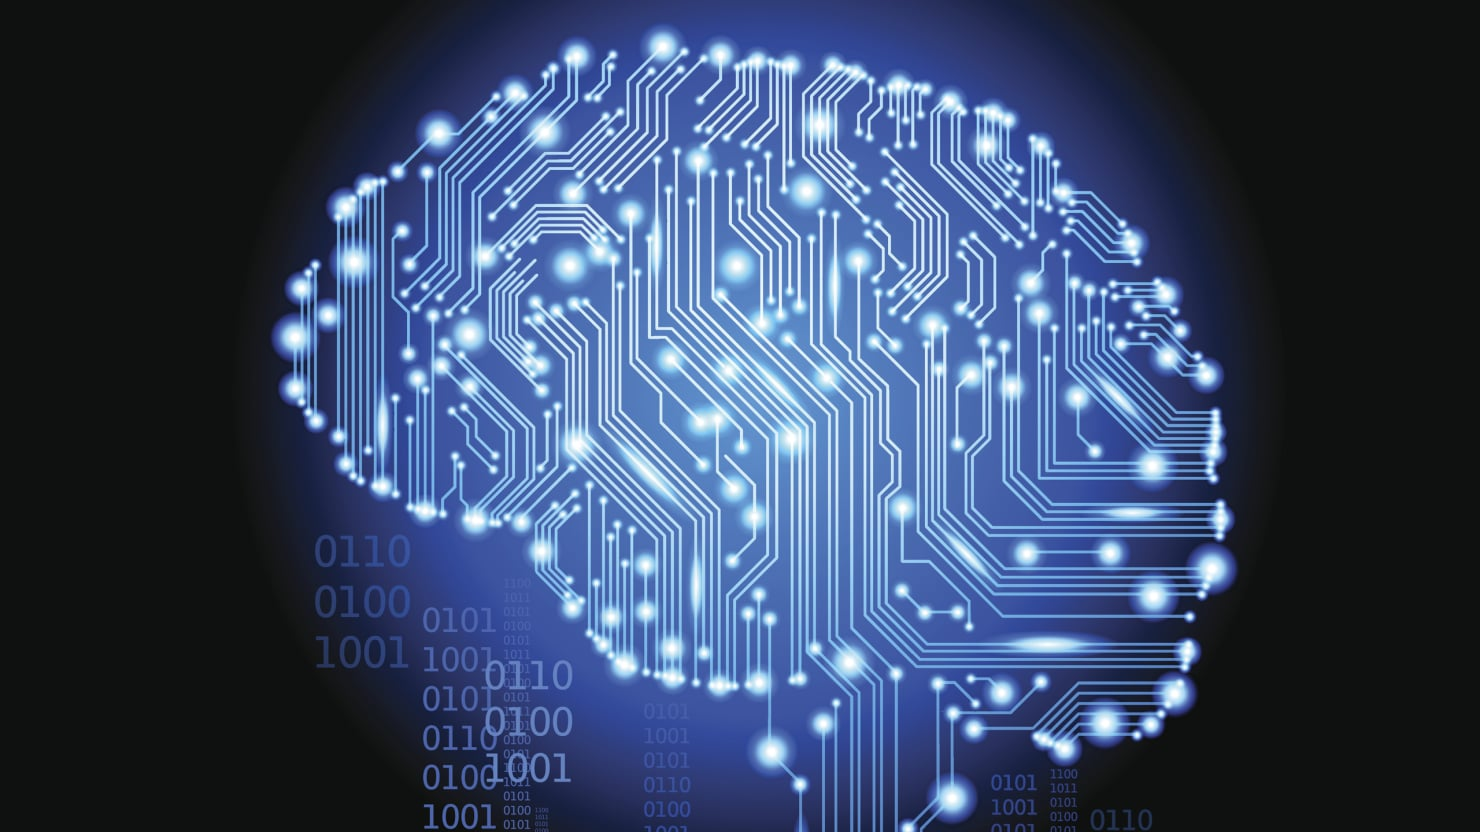
\includegraphics[width=\textwidth,height=0.7\textheight,keepaspectratio]{artificial-inteligence.jpg}
			\caption{Inteligencia Artificial}
		\end{figure}
		\column{.55\textwidth} % Left column and width
		\begin{itemize}
			\item \textbf{Opción 1:} Aplicar `nudges' para incrementar búsqueda de opciones de educacion superior:
					\begin{itemize}
					\item Reduciendo aversión al riesgo en la eleccion de carrera.
					\item Incentivando actitud positiva hacia a la educación.
					\end{itemize}

			\item \textbf{Opcion 2:} Proveer opción 1 mediante bot con Inteligencia Artificial:
					\begin{itemize}
					\item Bot aprende y predice preferencias personalizadas mediante interacción con el estudiante.
					\item Resultados más eficientes en términos de los retornos de elección de la carrera.
					\end{itemize}
		\end{itemize}
	\end{columns}
\end{frame} % -----------------------------------------------

\section{Ejemplo}
\stepcounter{subsection}
\begin{frame}{Ejemplo: Mensaje Inicial} % ---------------------------------[+2]
	\begin{textblock*}{1.5cm}(0.0005cm,7.65cm) % {block width} (coords)
		
\includegraphics[width=1.25cm]{header_foco.jpg}
	\end{textblock*}
	\begin{itemize}
		\item Hola, soy el Bot-ICFES! Estoy aquí para ayudarte. Existen más de 7,000 opciones de educación superior en Colombia. Afortunadamente, tengo una gran cantidad de información en mi cerebro que podría ayudarte a decidir. ¿Quisieras conversar conmigo sobre tu aplicación a la educación superior? No te preocupes por los costos del SMS, yo los tengo cubiertos.
	\end{itemize}
\end{frame} % -----------------------------------------------



\end{document}
